\chapter{Ricorsione}
	
	La ricorsione permette di definire nuovi valori di una funzione mediante vecchi valori. Tra queste funzioni, abbiamo la funzione fattoriale o la funzione per i numeri di Fibonacci.
	
	\section{Ricorsione primitiva}
	La definizione per ricorsione che useremo è la \textbf{ricorsione primitiva}. Siano $f(\vec{x})$ e $g(\vec{x},y,z)$ funzioni. Allora
	
	$$
	\begin{cases}
	h(\vec{x}, 0) = f(\vec{x})\\
	h(\vec{x}, y+1) = g(\vec{x}, y, h(\vec{x}, y))\\
	\end{cases}
	$$
	
	Costituisce una definizione per ricorsione di $h(\vec{x}, y)$ da $f(\vec{x}), g(\vec{x}, y, z)$. Le due equazioni sono dette \textbf{equazioni ricorsive}.
	
	\subsection{Teorema sull'esistenza e unicità}
	La precedente definizione trae forza dal seguente teorema. 
	Sia $\vec{x} = (x_1, \dots, x_n)$, e $f(\vec{x})$ e $g(\vec{x},y,z)$ funzioni. Allora esiste un'unica funzione $h(\vec{x}, y)$ che soddisfa le equazioni ricorsive
	
	
	\begin{itemize}
	\item $h(\vec{x}, 0) = f(\vec{x})$
	\item $h(\vec{x}, y+1)  = g(\vec{x}, y, h(\vec{x}, y))$
	\end{itemize}
	
	
	Inoltre, nel caso specifico di $\vec{x}$ assenti, e quindi arietà nulla, le equazioni ricorsive diventano
	
	$$
	\begin{cases}
		h(0) = a\\
		h(y+1) = g(y, h(y))\\
	\end{cases}
	$$
	
	\paragraph{Unicità} Siano $h'$ e $h''$ soddisfacenti le proprietà
	\begin{itemize}
		\item $h(\vec{x},0) = f(\vec{x})$
		\item $h(\vec{x}, y+1) = g(\vec{x},y,h(\vec{x},y))$
	\end{itemize}
	
	e tali che $h' \neq h''$. Sia $y$ il \textbf{minimo} per cui esista $\vec{x}$ tale che 
	$$
	h'(\vec{x},y) \neq h''(\vec{x}, y)
	$$
	
	Questo valore di $y$ deve essere maggiore (e non uguale) a 0, in quanto questo statement
	
	$$
	f(\vec{x}) = h'(\vec{x}, 0) \neq h''(\vec{x}, 0) = f(\vec{x})
	$$
	
	è ovviamente un assurdo. Sia dunque $y = y^*+1$, con $y^* \geq 0$. Pertanto, $h'(\vec{x}, y*) = h''(\vec{x}, y*)$, da cui
	
\begin{align*}
	h'(\vec{x}, y) &= h(\vec{x}, y^*+1)\\ 
	&= g(\vec{x}, y^*, h'(\vec{x}, y^*))\\ 
	&= g(\vec{x}, y^*, h''(\vec{x}, y^*))\\ 
	&= h''(\vec{x}, y^*). \quad \textbf{Contraddizione!}\\ 
\end{align*}
$h' = h''$. 
Quindi, se esiste una funzione $h$ che soddisfa delle date equazioni ricorsive, questa è unica.
	
	
	\paragraph{Esistenza} La dimostrazione dell'esistenza è data per buona, in quanto molto complessa da affrontare.
	
	\subsection{Esempi di funzioni calcolabili con ricorsione primitive}
	
	Addizione, moltiplicazione, fattoriale. \verb|TODO|.
	
	\subsection{Teorema sulla calcolabilità della ricorsione primitiva}
	Se $f(\vec{x})$ e $g(\vec{x}, y, z)$ sono calcolabili, anche la funzione $h(\vec{x},y)$  definita per ricorsione primitiva con $f(\vec{x})$ e $g(\vec{x},y,z)$ come equazioni ricorsive, è calcolabile.
	
	\paragraph{Dimostrazione} Siano $F$ e $G$ programmi in \textbf{forma standard} che calcolano rispettivamente $f$ e $g$. 
	Poniamo $m=\max(\rho(F), \rho(G), n+2)$, ove $\vec{x}=(x_1, \dots, x_n)$. È facile convincersi che il seguente programma calcola la funzione $h(\vec{x}, y)$.
	
	\begin{algorithm}
		\caption{\textit{Ricorsione primitiva}}
		\begin{algorithmic}
			\State $T(1, m+1)$
			\State \qquad\vdots
			\State $T(n+1, m+n+1)$ \Comment{Copia l'input in un'area sicura}
			\State $R_{m+n+3} \leftarrow f_F^{(n)} (R_{m+1}, \dots, R_{m+n})$ \Comment{Calcola il caso base}
			\State [$I_q$]:
			\State $J(m+n+2, m+n+1, p)$ \Comment{Condizione di uscita dalla ricorsione}
			\State $R_{m+n+3} \leftarrow f_G^{(n+2)} (R_{m+1}, \dots, R_{m+n}, R_{m+n+2}, R_{m+n+3})$
			\State $S(m+n+2)$
			\State $J(1,1,q)$ \Comment{while True}
			\State $[I_p]: \ T(m+n+3, 1)$
		\end{algorithmic}
	\end{algorithm}
	
	Il registro $R_{m+n+1}$ contiene il numero di passi ricorsivi da fare, con $R_{m+n+2}$ usato come contatore.
	
	
	\section{Funzioni primitive ricorsive}
	Abbiamo dimostrato, fino ad ora, che le funzioni iniziali sono calcolabili, le composizioni di funzioni calcolabili sono calcolabili, e che \textbf{la ricorsione primitiva} su funzioni calcolabili dà luogo a funzioni \textbf{calcolabili}. Chiameremo \textbf{primitive ricorsive} le funzioni ottenute a partire da funzioni iniziali tramite un numero finito di composizioni e ricorsioni primitive. Denotiamo l'insieme delle primitive ricorsive $\mathcal{PR}$.
	
	

	
	\subsection{Insieme $\mathcal{PR}$}
	
	Non tutte le funzioni URM-calcolabili appartengono all'insieme delle funzioni primitive ricorsive. La minimalizzazione (non limitata) ci permetterà di ottenere funzioni molto più espressive, permettendoci di solcare anche il suolo delle funzioni parziali \textbf{non totali}. 
	
	\begin{figure}[tbph]
		\centering
		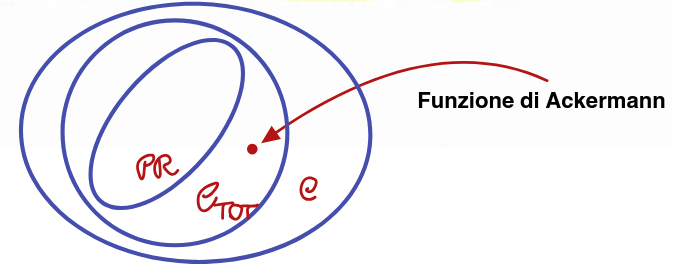
\includegraphics[width=0.75\linewidth]{images/insiemi-ricorsive-calcolabili}
		\caption{Le funzioni $\mathcal{PR}$ non coprono tutte le funzioni calcolabili totali, e in particolare, nessuna funzione parziale \textbf{non totale} è primitiva ricorsiva.}
	\end{figure}
	